\section{The Vending Machine Example}\label{sec:example}

To illustrate the \toolname's functionalities we will use a simple
example, adapted from~\cite{Orso01UCMS}, consisting of a component
and an application that uses it. Figure~\ref{fig:vending} shows
the Java source code of the \pk{VendingMachine} application and of
the \pk{Dispenser} component. Although \toolname does not require
the source code available to perform its operations, we show it
here to ease the understanding of the vending machine application.

This source code implements a typical vending machine that is able
to dispense specific items to a customer under certain conditions.
The basic operations that a given customer may perform are: (1) to
insert a coin of 25 cents into the machine
(\pk{VendingMachine.inservCoin()}); (2) to ask the machine to
return the inserted and not consumed coins
(\pk{VendingMachine.returnCoin()}); and (3) to ask the machine to
vend a specific item (\pk{VendingMachine.vendItem()}). The
\pk{Dispenser} component keeps information about the price of each
item and which items are valid and available. The basic steps
performed by the \pk{Dispenser} component are:

\begin{enumerate}
    \item Checks if at least one coin have been inserted;
    \item Checks if a valid item have been selected;
    \item Checks if the valid item selected is available;
    \item Checks if the credit is enough to buy the valid
    available selected item.
\end{enumerate}

Different error messages are generated by the \pk{Dispenser}
component in case the pre-requirements to delivered a given item
are not satisfied. \pk{Dispenser}'s source code lines 16, 18, 20
and 24 illustrates these messages.

In case all pre-requirements are satisfied, the message at source
line 26 is displayed indicating that the operation was performed
successfully. Observe that the vector of integers
\pk{availSelectionVals} (\pk{Dispeser}'s source line 08) defines
the current set of valid and available items. For example,
according to \pk{availSelectionVals}, items 5, 18 and 20 are
unavailable. Such a vector can be updated by calling the
\pk{Dispeser.setValidSelection()} method (\pk{Dispeser}'s source
line 42).

\begin{figure}[!ht]
\begin{center}
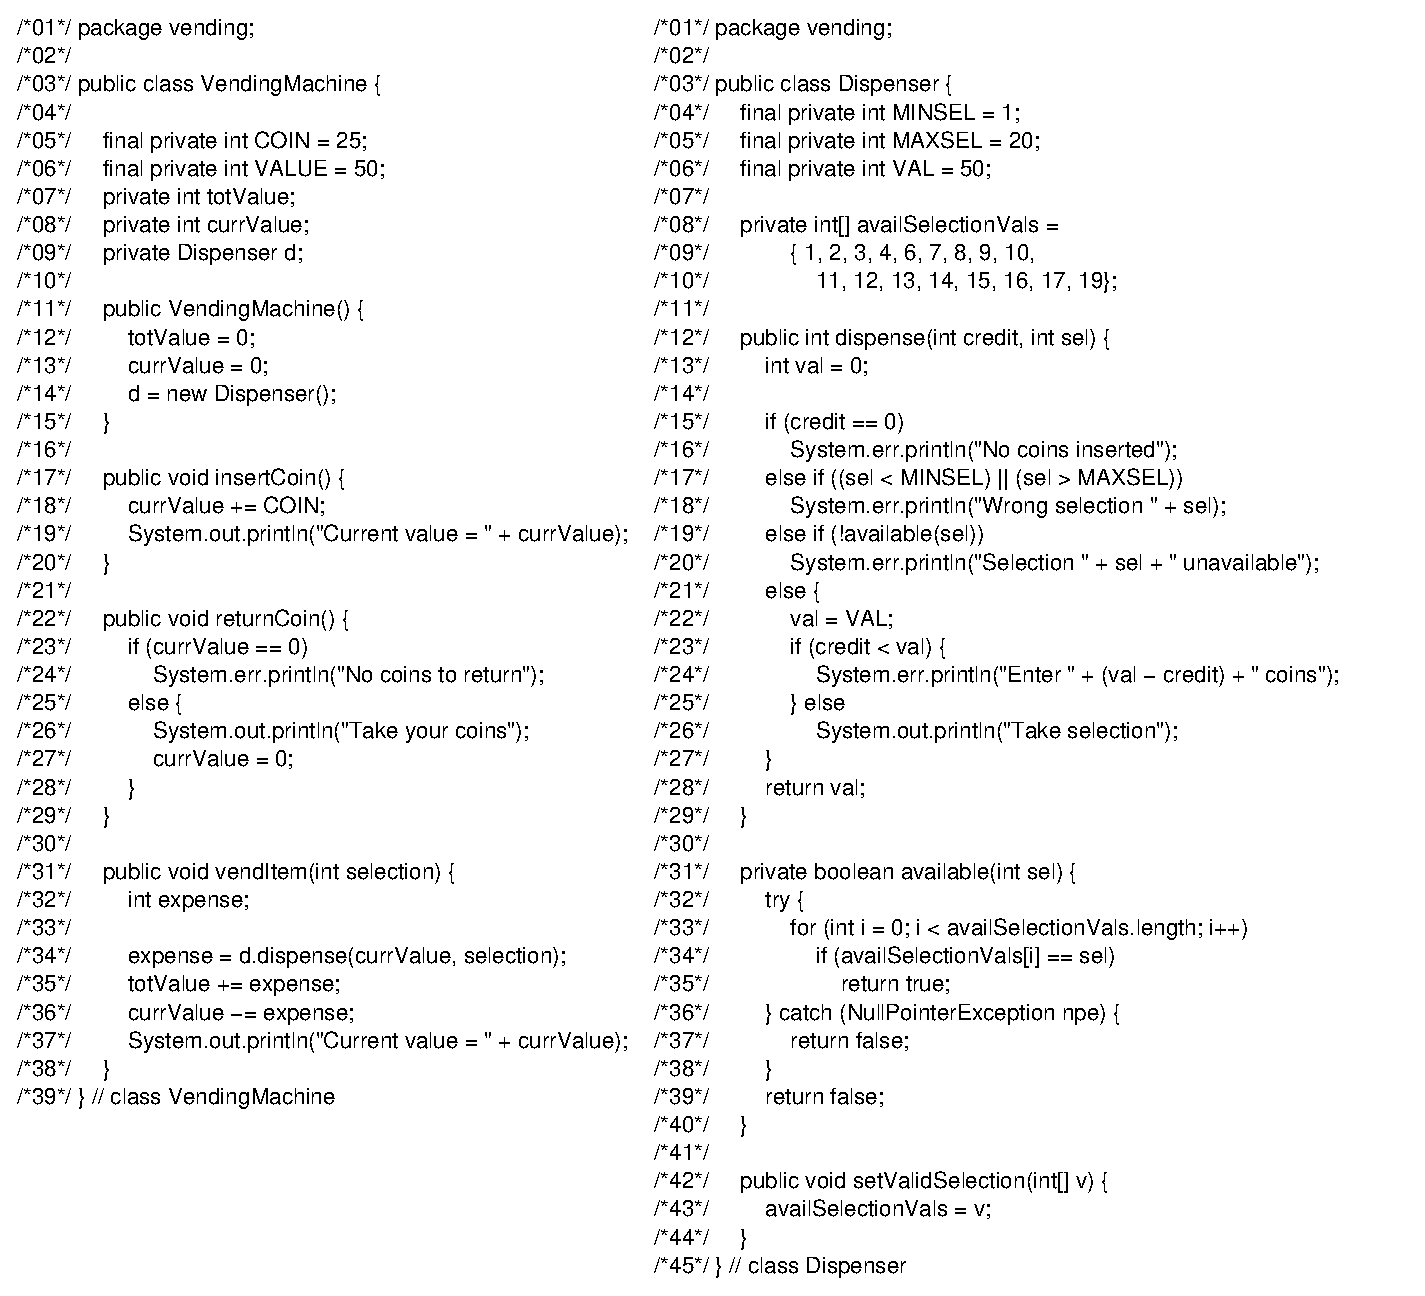
\includegraphics[width=\textwidth]{fig/vending-dispenser.eps}
\caption{\label{fig:vending}Example adapted from~\cite{Orso01UCMS}
of a Java application (\pk{VendingMachine}) and one component
(\pk{Dispenser}).}
\end{center}
\end{figure}


Since neither \pk{VendingMachine} nor \pk{Dispenser} classes have
a \pk{main} method, to allow the invocation of each method of the
\pk{VendingMachine} class, we developed a test driver class
(\pk{TestDriver}) that accepts as input a text file containing a
set of methods' names that have to be executed in the
\pk{VendingMachine} class, creates an instance of
\pk{VendingMachine}, and perform the execution of the required
methods. Figure~\ref{fig:drv} shows the source code of the test
driver.

\begin{figure}[!ht]
\begin{center}
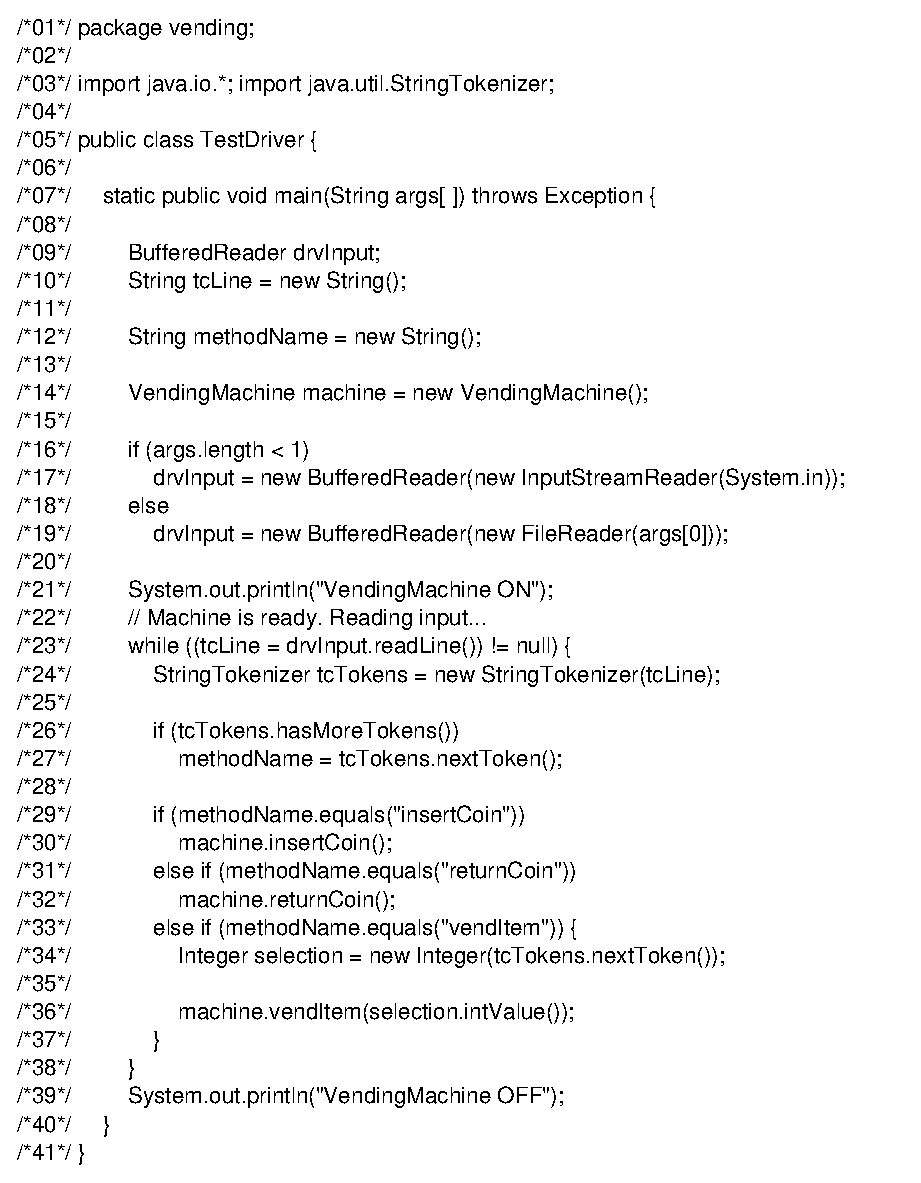
\includegraphics[width=0.6\textwidth]{fig/testdriver.eps}
\caption{\label{fig:drv}Example of a test driver for
\texttt{VendingMachine} and \texttt{Dispenser} classes.}
\end{center}
\end{figure}


For example, considering a typical execution of the vending
machine, a customer insert a certain number of coins, ask to the
vending machine to deliver a given item, and the vending machine
dispenses the required item if it is valid and available. This
steps can be represented by a text file \pk{input1}
(Figure~\ref{fig:input}).

\begin{figure}[!ht]
\begin{cmd}
        insertCoin
        insertCoin
        vendItem 3
\end{cmd}
\vspace{-0.7cm}\caption{A simple test case file:
\pk{input1}.}\label{fig:input}
\end{figure}

By executing the command illustrated in Figure~\ref{fig:driver},
\pk{input1} is read line by line. The first two lines cause the
execution of the method \pk{VendingMachine.insertCoin} twice,
indicating that the customer deposited 50 cents into the vending
machine. The last line corresponds to the choice to buy the item
number three, a valid item that will be delivered to the customer.
Using this approach, valid and invalid test cases can be specified
to check whether the \pk{VendingMachine} application and the
\pk{Dispenser} component behave correctly \wrt their
specifications.

\begin{figure}[!ht]
\begin{cmd}
        java vending.TestDriver input1
\end{cmd}
\vspace{-0.7cm}
\caption{How to execute the implemented test
driver.}\label{fig:driver}
\end{figure}

\rev{Orso \etal~\cite{Orso01UCMS} comment that the source code
presented in Figure~\ref{fig:vending} contains a fault in method
\pk{Dispenser.dispense()}: when a available item is selected and
the credit is insufficient, but greater than zero, the variable
\pk{val} (set to \pk{VAL} at line 22 of \pk{Dispenser} class) is
not set to zero; consequently, when control returns from
\pk{Dispenser.dispense()} to \pk{VendingMachine.vendItem()},
\pk{currValue} is erroneously decremented. To fix this error, the
statement \pk{val = 0} should be included after the statement
located at \pk{Dispenser.dispense()}'s source line 24. Observe
that we will use the faulty version of the \pk{Dispenser}
component to show how the slicing tool (described in
Section~\ref{sec:slice}) can be used to help the localization of
such a fault.}
